\section{Benchmark Dataset}

Datasets play a crucial role in developing and evaluating Text-to-SQL models for semantic parsing of natural language phrases. A variety of benchmark datasets are available, each with unique characteristics and features. Examples of early datasets include ATIS\cite{dahl-etal-1994-expanding}, GeoQuery\cite{10.1007/3-540-44795-4_40}, and Yelp\cite{10.1145/3133887}, which focus on a single topic and database. More recent datasets, such as WikiSQL\cite{zhong_seq2sql_2017} and Spider\cite{yu_spider_2019}, are larger and cover a broader range of domains.

Additionally, new datasets include more advanced queries to assess the generalization capabilities of models. These benchmark datasets provide a standardized testbed for evaluating the performance of Text-to-SQL models and are widely used in the research community. They vary in complexity, size, and annotation, allowing researchers to evaluate models' performance at different levels and under different scenarios. This chapter will review the top benchmark datasets used in the Text-to-SQL Semantic Parsing community and discuss their significance for the research community.

\subsection{Single-Domain}

\subsubsection{ATIS (Air Travel Information System) and GeoQuery}

ATIS (Air Travel Information System)\cite{dahl-etal-1994-expanding} and GeoQuery\cite{10.1007/3-540-44795-4_40} are two datasets that are frequently utilized for semantic parsing, a technique for converting natural language inquiries into a structured meaning representation. The ATIS dataset consists of audio recordings and hand transcripts of individuals using automated travel inquiry systems to search for information regarding flights. It is structured using a relational schema to organize data from the official airline guide, with 25 tables containing information concerning fares, airlines, flights, cities, airports, and ground services.
All questions concerning this dataset can be answered using a single relational query. This makes it an ideal choice for training deep learning models, as it is designed for a specific domain and the queries are relatively straightforward.

Furthermore, the questions in the ATIS dataset are mainly limited to select and project queries. On the other hand, GeoQuery is made up of seven tables from the US geography database and 880 natural languages to SQL pairings. It includes geographic and topographical characteristics such as capitals, populations, and landforms. While both datasets are regularly employed to train deep learning models, GeoQuery is more comprehensive and provides a wider range of queries than ATIS. This includes join and nested queries, as well as grouping and ordering queries, which are absent in the ATIS dataset. As a result, GeoQuery is better equipped to answer more complex queries, making it a better choice for training AI models.

% A relational schema is used to organize data from the official airline guide in the ATIS corpus. There are 25 tables containing information about fares, airlines, flights, cities, airports, and ground services. All questions related to this dataset can be answered using a single relational query. The relational database uses shorter tables for this dataset to answer queries intuitively.

% Here is an example query from the ATIS dataset: Input is in natural language, and the output is in \lambda calculus.

% \begin{figure}[htb]
%     \centering
%     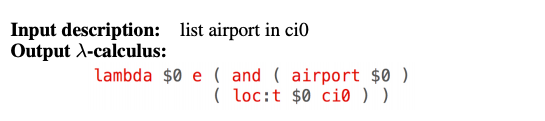
\includegraphics[width=0.8\textwidth]{pics/db/ATIS.png}
%     \caption{Example from ATIS dataset for semantic parsing}
%     \label{fig:ATIS}
% \end{figure}

% \subsubsection{GeoQuery Dataset}

% United States geography is represented in the Geoquery dataset. About 800 facts are expressed in Prolog. State, city, river, and mountain information can be found in the database. Geographic and topographical attributes such as capitals and populations make up the majority of the attributes.

\subsubsection{IMDb Dataset}

The IMDb dataset is a well-known dataset in the machine learning community. It contains 50,000 reviews from IMDb and has a limit of 30 reviews per movie\cite{maas-EtAl:2011:ACL-HLT2011}. It is noteworthy that the dataset is balanced in terms of positive and negative reviews, which are equally represented. When creating the dataset, reviews with a score of 4 out of 10 were considered negative and those with a score of 7 out of 10 were considered positive. Neural reviews were excluded to maintain the quality of the dataset. The dataset is divided into training and testing datasets, each with an equal portion. To ensure fairness and accuracy in the results, the dataset creators have taken special care to keep the training and testing datasets balanced.

\begin{figure}[htb]
    \centering
    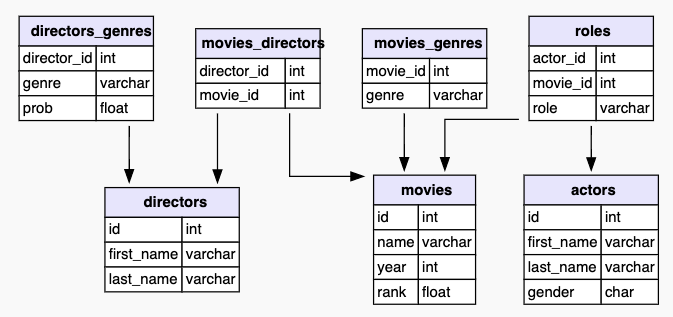
\includegraphics[width=0.8\textwidth]{pics/db/IMDb.png}
    \caption{Database Structure of IMDb dataset\cite{dahl-etal-1994-expanding}}
    \label{fig:IMDb}
\end{figure}

% \newpage % to avoid page break

\subsubsection{Advising Dataset}

The Advising dataset\cite{finegan-dollak-etal-2018-improving} was created in order to propose improvements in Text-to-SQL systems. The creators of the dataset compare human-generated and automatically generated questions, citing properties of queries that relate to real-world applications. The dataset consists of questions from the University of Michigan students about courses that lead to particularly complex queries. The data is obtained from a fictional student database which includes student profile information such as recommended courses, grades, and previous courses. Moreover, in order to obtain the data for the dataset, academic advising meetings were conducted where students were asked to formulate questions they would ask if they knew the database. After obtaining the questions, the creators of the dataset compared the query results with those from other datasets such as ATIS, GeoQuery, and Scholar. Many of the queries in the Advising dataset were the same as those found in the other datasets.

% \begin{figure}[htb]
%     \centering
%     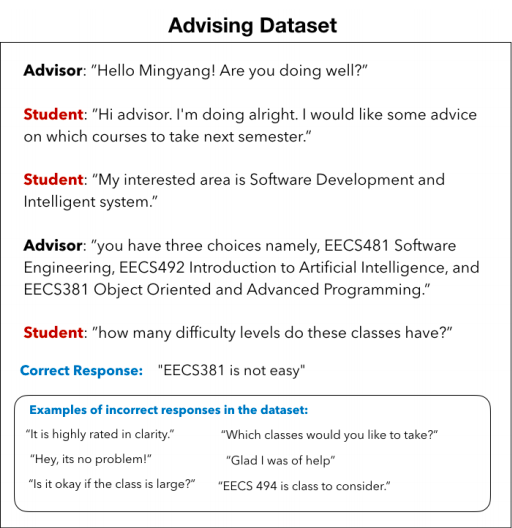
\includegraphics[width=0.5\textwidth]{pics/db/Advising.png}
%     \caption{Example from Advising dataset \cite{vig_comparison_2019}}
%     \label{fig:Advising}
% \end{figure}

\subsubsection{MAS (Microsoft Academic Search)}

MAS, or Microsoft Academic Search\cite{roy2013the}, is a database of academic and social networks and a collection of queries. It has a total of 17 tables in its database, as well as 196 natural languages to SQL pairs. MAS can handle join, grouping, and nested queries but does not support ordering queries.

There are a few limitations to be aware of when using natural language queries within MAS. Firstly, all-natural language questions must begin with the phrase ”return me” and can not include an interrogative statement or a collection of keywords. Additionally, all queries must follow the proper grammatical conventions.

\clearpage

\subsection{Large Scale Cross-Domain}

\subsubsection{WikiSQL}

WikiSQL consists of 80,654 natural language questions and corresponding SQL queries on 24,241 tables extracted from Wikipedia. Neither the train nor development sets contain the database in the test set. Databases and SQL queries have simplified the dataset's creators' assumptions. This dataset consists only of SQL labels covering a single SELECT column and aggregation and WHERE conditions. Furthermore, all the databases contain only one table.

The database does not include complex queries involving advanced operations like JOIN, GROUP BY, ORDER BY, etc. Prior to the release of SPIDER, this dataset was considered to be a benchmark dataset. Using WikiSQL has been the subject of a great deal of research. WikiSQL's "WHERE" clause has been recognized as one of the most challenging clauses to parse semantically, and SQLNet and SyntaxSQL were previous state-of-the-art models.


\begin{figure}[htb]
    \centering
    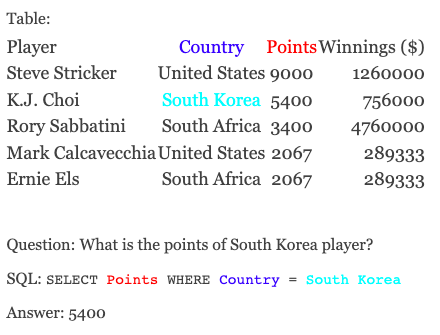
\includegraphics[width=0.5\textwidth]{pics/db/WikiSQL.png}
    \caption{Example from WikiSQL dataset\cite{DBLP:journals/corr/abs-1902-01069}}
    \label{fig:WikiSQL}
\end{figure}

The WikiSQL challenge is a research competition focused on developing natural language interfaces for databases. The challenge includes several state-of-the-art Text-to-SQL solutions proposed by different research teams.

One example of a state-of-the-art Text-to-SQL solution in the WikiSQL challenge is the Seq2SQL model, which uses a sequence-to-sequence learning framework to map natural language input to SQL queries. The model uses an attention mechanism to align the input and output sequences and a pointer network to handle SQL queries with complex structural dependencies.

Another example is the Spider model, which uses a combination of recurrent and convolutional neural networks to learn the mapping between natural language and SQL queries. The model uses a hierarchical structure to process the natural language input, with separate modules for understanding the query's intent, columns, and constraints.
One difference between these research approaches is the specific deep learning architecture used. The Seq2SQL model uses a sequence-to-sequence framework, while the Spider model uses a combination of RNNs and convolutional neural networks. Additionally, the Spider model uses a hierarchical structure to process the natural language input, while the Seq2SQL model processes the input linearly.

Another difference is in the evaluation metrics used. The Seq2SQL model is evaluated using the execution accuracy of the generated SQL queries, while the Spider model is evaluated using a combination of execution accuracy and natural language understanding metrics.
Overall, both the Seq2SQL and Spider models are state-of-the-art Text-to-SQL solutions that have achieved high performance in the WikiSQL challenge. However, their specific architectures and evaluation metrics differ, which can affect their performance and accuracy on different tasks.
\subsubsection{SPIDER}

The SPIDER database contains 10K questions and 5K+ complex SQL queries covering 138 different domains across 200 databases. As opposed to previous datasets (most of which used only one database), this one incorporates multiple datasets. Creating this dataset took 11 Yale University students, 1,000 man-hours in total.

Spider contains queries with a lot of intricate SQL elements. In comparison to the sum of the previous Text-to-SQL datasets, Spider comprises around twice as many nested queries and ten times as many ORDER BY (LIMIT) and GROUP BY (HAVING) components.

Creating this corpus was primarily motivated by the desire to tackle complex queries and generalize across databases without requiring multiple interactions.

\begin{figure}[htb]
    \centering
    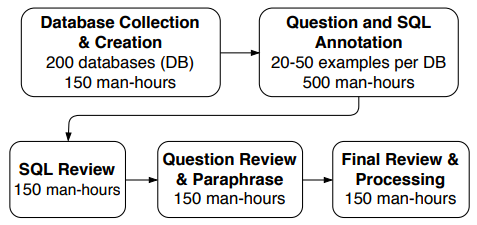
\includegraphics[width=0.6\textwidth]{pics/db/Spider.png}
    \caption{Process of creating SPIDER dataset\cite{yu_spider_2019}}
    \label{fig:Spider}
\end{figure}

Creating a dataset involves three main aspects: SQL pattern coverage, SQL consistency, and question clarity. Several databases from WikiSQL are included in the dataset. The table is complex as it links several tables with foreign keys. In SPIDER, SQL queries include: SELECT with multiple columns and aggregations, WHERE, GROUP BY, HAVING, ORDER BY, LIMIT, JOIN, INTERSECT, EXCEPT, UNION, NOT IN, OR, AND, EXISTS, LIKE.

The complexity of the dataset increases and the accuracy of solutions drops as the number of foreign keys in the database increases. This is mainly due to the difficulty in selecting the relevant column and table names from a complex database schema. Furthermore, complex database schemas present a major challenge for the model to accurately capture the relationship between different tables which involve foreign keys. SQL queries with a higher number of foreign keys tend to join more tables, suggesting a need for more effective methods to encode the connection between tables with foreign keys.

\subsubsection*{SQL Hardness Criteria}

In order to gain a better understanding of how the model performs on different queries, we have divided SQL queries into four difficulty levels: easy, medium, hard, and extra hard. This classification is based on the number of SQL components, selections, and conditions. Queries that contain multiple SQL keywords (e.g., GROUP BY, ORDER BY, INTERSECT, nested subqueries, column selections, aggregators) are generally considered more complex. For example, a query is considered hard if it includes more than two SELECT columns, more than two WHERE conditions, and GROUP BY two columns, or contains EXCEPT or nested queries. If it contains even more additions on top of that, it is considered extra hard.

\begin{figure}[htb]
    \centering
    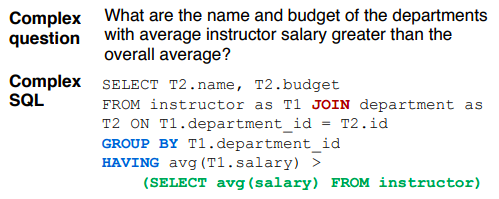
\includegraphics[width=0.8\textwidth]{pics/db/Spider2.png}
    \caption{Example of Question-Query set from SPIDER\cite{yu_spider_2019}}
    \label{fig:Spider2}
\end{figure}


SPIDER's exact matching accuracy\ref{eval} was 12.4\% compared to existing state-of-the-art models. As a result of its low accuracy, SPIDER presents a strong research challenge. Current SPIDER accuracy is above 75.5\% with an exact set match without values (refers to values in the WHERE clause) and above 72.6\% with values using PICARD\ref{picard}.

The SPIDER challenge is a research competition dedicated to developing cutting-edge Text-to-SQL and Semantic Parsing solutions. In this challenge, participants strive to develop algorithms that can automatically generate structured SQL queries from natural language input, to improve the performance and accuracy of Text-to-SQL models.

In this challenge, numerous state-of-the-art Text-to-SQL solutions have been proposed, such as the Spider model. This model uses a combination of recurrent and convolutional neural networks to learn the mapping between natural language and SQL queries. This model also has a hierarchical structure, which allows it to process the natural language input more effectively, thereby allowing it to handle complex queries and variations in language with greater precision and accuracy. This model successfully generates accurate and efficient SQL queries from natural language inputs.

One difference between the SPIDER and WikiSQL challenges is the specific dataset that is used for evaluation. The SPIDER challenge uses a dataset of complex SQL queries and natural language questions derived from real-world databases, while the WikiSQL challenge uses a dataset of more straightforward SQL queries and natural language questions derived from Wikipedia articles. This difference in the dataset can affect the performance and accuracy of the models on the different tasks.

Another difference is in the evaluation metrics used. The SPIDER challenge evaluates the models using execution accuracy and natural language understanding metrics, while the WikiSQL challenge evaluates the models using only execution accuracy. This difference in the evaluation metrics can affect how the models are trained and their performance on the tasks. We will discuss the evaluation metrics used in the SPIDER challenge in more detail in the next section\ref{eval}.
\subsubsection{SEDE}

\ac{SEDE} \cite{DBLP:journals/corr/abs-2106-05006} is from a popular online question-and-answer platform with more than 3 million questions, and it recently released a benchmark dataset of SQL queries containing 29 tables and 211 columns. This dataset comprises real-world questions from the Stack Exchange website, such as published posts, comments, votes, tags, and awards.

Although these datasets contain a variety of real-world challenges, they still need to be more tricky to parse semantically due to the complexity of the questions they contain. After further analysis of the 12,023 questions asked on the platform, a total of 1,714 have been verified by humans, which makes it an ideal choice for training and validating the model. This benchmark dataset is highly valuable and helpful for research in natural language processing, as it provides an extensive list of real-world challenges that have rarely been seen in other semantic parsing datasets.

\begin{figure}[H]
    \label{fig:sede_sql}
    \begin{AIbox}{An example of a Complex SEDE utterance}
        \vspace{-5px}
        \parbox{1\textwidth}{\scriptsize
        \begin{alltt} \larger
            {\bf Utterance:} \\ 
            Check if Votes.CreationDate is always a date
            \\
            {\bf Query:} \\
            SELECT Name, Count(*)as [Count], DatePart(Hour, Votes.CreationDate)as [hour],DatePart(Minute, Votes.CreationDate)as [minute],DatePart(Second, Votes.CreationDate)as [second],DatePart(Millisecond, Votes.CreationDate)as [ms] FROM Votes JOIN VoteTypes ON VoteTypeId = VoteTypes.Id GROUP BY Name, DatePart(Hour, Votes.CreationDate),DatePart(Minute, Votes.CreationDate),DatePart(Second, Votes.CreationDate),DatePart(Millisecond, Votes.CreationDate)
        \end{alltt}
        }
        \vspace{-5px}
    \end{AIbox}
    
    \captionsetup{font={scriptsize,color=white}, skip=-20pt}
    \caption{An example of a Complex SEDE utterance}
\end{figure}
\subsubsection{SEOSS}

\ac{SEOSS} dataset is a compilation of natural language expressions with seven alternative phrasings, each linked to a single SQL query. In total, 166 questions (expressions) were organized. The natural language expressions were mainly obtained from existing literature and modified to match the data identified in the issue tracking system (ITS) and version control system (VCS) of an existing software project (namely Apache Pig). This data was extracted and saved into an SQLite database by Rath et al. \cite{RATH2019104005}.

\begin{figure}[H]
    \centering
    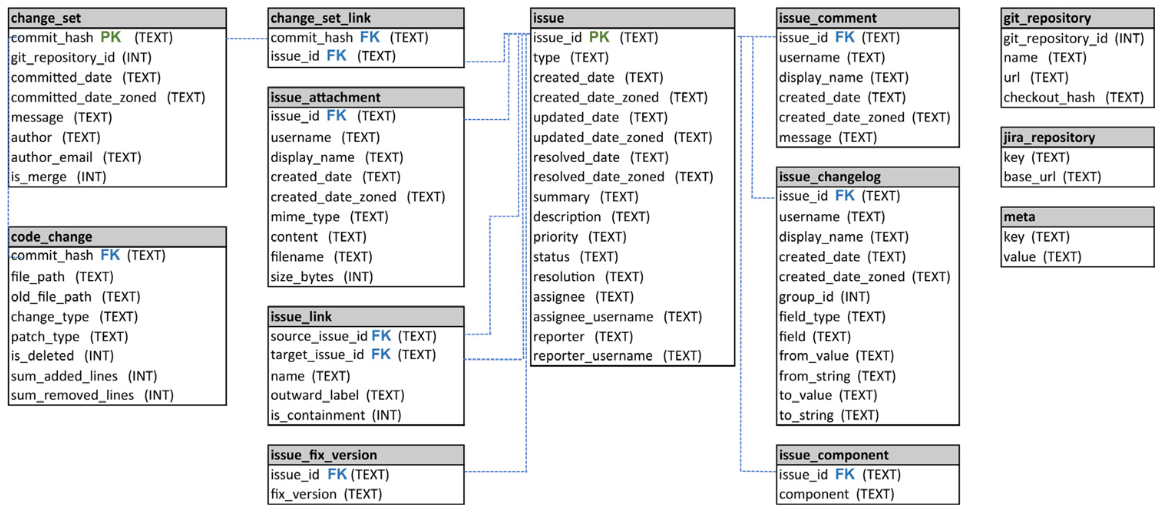
\includegraphics[width=1\textwidth]{pics/seoss/pig.png}
    \caption{Database Schema of the PIG Database \cite{TOMOVA2022108211}}
    \label{fig:SESS}
\end{figure}

Expressions are labeled into two different tags, development and research. Eighty-one queries with a focus on software needs of stakeholders and developers or from typical use cases' queries of issue tracking systems were labeled as 'development,' and 63 queries containing issue tracking systems information or version control systems were labeled as 'research.' Also, 22 records were generated from the content in questions stakeholders asked within the comment sections of issues of type bug, enhancement/improvement, new feature/feature request, and tasks of 33 open-source Apache projects, which were extracted and stored into databases by Rath and Mäder\cite{RATH2019104005}.
In SEOSS-Queries\cite{TOMOVA2022108211} research, they experienced RatSQL and SQLNet methods on the SEOSS dataset and released their evaluation steps. In this research, we will use the same dataset to evaluate state-of-the-art models currently available in the literature and used in SPIDER for this dataset.


% TODO: need more about the Hardness of the SEOSS dataset
% \begin{figure}[H]
%     \centering
%     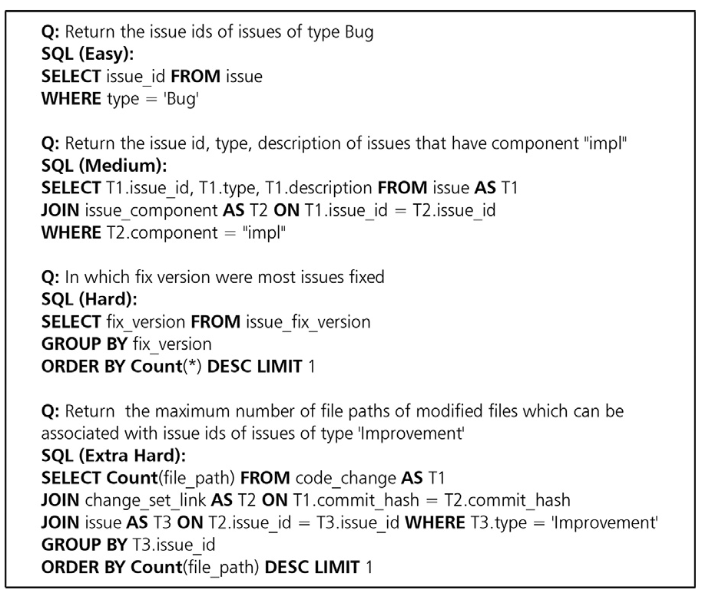
\includegraphics[width=0.8\textwidth]{pics/seoss/seoss.png}
%     \caption{\small Examples of queries with different levels of complexity in SEOSS-Queries \cite{TOMOVA2022108211}}
%     \label{fig:SESS2}
% \end{figure}

\begin{figure}[H]
    \label{fig:SESS2}
    \begin{AIbox}{An example of an extra-hard SEOSS record}
        \vspace{-5px}
        \parbox{1\textwidth}{\scriptsize
        \begin{alltt} \larger
            {\bf Utterance:} \\ 
            Return  the maximum number of file paths of modified files which can be associated with issue ids of issues of type 'Improvement
            \\
            {\bf Query:} \\
            SELECT Count(file\_path) FROM code\_change AS T1 JOIN change\_set\_link AS T2 ON T1.commit\_hash = T2.commit\_hash JOIN issue AS T3 ON T2.issue\_id = T3.issue\_id WHERE T3.type = 'Improvement' GROUP BY T3.issue\_id ORDER BY Count(file\_path) DESC LIMIT 1
        \end{alltt}
        }
        \vspace{-5px}
    \end{AIbox}
    
    \captionsetup{font={scriptsize,color=white}, skip=-20pt}
    \caption{An example of an extra-hard SEOSS record}
\end{figure}



% \clearpage

In this chapter, we have reviewed various datasets widely used in the Text-to-SQL Semantic Parsing community. These datasets vary in complexity, size, and annotation, providing a standardized testbed for evaluating the performance of Text-to-SQL models. We have discussed their unique characteristics and features from early datasets such as ATIS and GeoQuery to more recent datasets such as WikiSQL and Spider.
The datasets discussed in this chapter are a valuable resource for the research community to evaluate the progress and performance of Text-to-SQL models. The continued development and improvement of these datasets will be necessary for advancing the field of Text-to-SQL Semantic Parsing.
The table\ref{tab:datasets} below provides an overview of the datasets mentioned in this chapter, including the number of queries and questions sorted by year.

\begin{table}[!ht]
    \centering
    \begin{tabular}{|c|c|c|c|c|c|c|}
        \hline
        \textbf{Dataset} & \textbf{Year} & \textbf{DBs} & \textbf{Tables} & \textbf{Utterances} & \textbf{Queries} & \textbf{Domain}            \\ \hline
        ATIS             & 1994          & 1            & 32              & 5280                & 947              & Air Travel Information     \\ \hline
        GeoQuery         & 2001          & 1            & 6               & 877                 & 247              & US geography database      \\ \hline
        Academic         & 2014          & 1            & 15              & 196                 & 185              & Microsoft Academic Search  \\ \hline
        IMDB             & 2015          & 1            & 16              & 131                 & 89               & Internet Movie Database    \\ \hline
        Scholar          & 2017          & 1            & 7               & 817                 & 193              & Academic Publications      \\ \hline
        Yelp             & 2017          & 1            & 7               & 128                 & 110              & Yelp Movie Website         \\ \hline
        WikiSQL          & 2017          & 26.521       & 26,521          & 80,654              & 77,840           & Wikipedia                  \\ \hline
        Advising         & 2018          & 1            & 10              & 3,898               & 208              & Student Course Information \\ \hline
        Spider           & 2018          & 200          & 1,020           & 10,181              & 5,693            & 138 Different Domains      \\ \hline
        SEDE             & 2021          & 1            & 29              & 12,023              & 11,767           & Stack Exchange             \\ \hline
        SEOSS            & 2022          & 1            & 13              & 1,162               & 116              & Project ITS and VSC        \\ \hline
    \end{tabular}
    \caption{Comparison of datasets (Sort by Year)}
    \label{tab:datasets}
\end{table}
